\section{Completed four-arm spatial comparison}

\label{sec:s03-completed}

\textit{Numerical status: all folds passed their saved custody and score-decomposition checks, and the predeclared independent California-fold sample passed. Acceptance uses sampled validation, not independent raw replay of every fit.}

The comparison contains three California folds with 315 targets and three New Zealand folds with 612 targets. Four procedures are evaluated in each fold: arm 1 uses the reference-density-weighted rational offspring kernel and inherited KDE background; arm 2 removes reference-density weighting; arm 3 adds identity-based leave-one-out background fitting; arm 4 uses the unweighted EP offspring shape with the inherited background procedure. The temporal and mark parameters remain training-selected and fixed. Background level, trend and reproduction coefficient are refitted under the declared arm-specific normalization. California uses the archived training-selected EP spatial scale and shape. The New Zealand OC archives did not contain EP spatial parameters, so a separate training-only prerequisite estimated these missing nuisance parameters before the four-arm comparison. Those values were then frozen: each final arm optimizes only background level, trend and reproduction coefficient. This prerequisite is an explicit addition to the original execution specification, not a claim that the entire preparation fitted only three parameters.

\begin{table}[htbp]\centering

\caption{Held-out joint log-score contrasts in nats. Positive values favour the first named arm. Arm labels follow the text.}\label{tab:s03-completed}

\begin{tabular}{llrrrrr}\toprule Region & Fold & Targets & $2-1$ & $3-2$ & $4-2$ & $4-1$\\\midrule

CA & 0 & 79 & -0.2962 & 1.4515 & 6.3629 & 6.0668 \\

CA & 1 & 167 & 1.0722 & 3.1070 & 29.9884 & 31.0606 \\

CA & 2 & 69 & 0.2776 & 0.7288 & 12.6035 & 12.8811 \\

NZ & 0 & 203 & 0.3421 & 2.1881 & 17.9074 & 18.2495 \\

NZ & 1 & 155 & 33.2980 & -0.3822 & -0.0583 & 33.2397 \\

NZ & 2 & 254 & -1.2518 & -3.2235 & 0.0346 & -1.2172 \\

\bottomrule\end{tabular}\end{table}

\begin{table}[htbp]\centering

\caption{Regional totals for EP minus the OC baseline, in nats. The common mark score cancels.}

\begin{tabular}{lrrr}\toprule Region & Timing & Location & Joint\\\midrule

CA & -0.8205 & 50.8289 & 50.0085 \\

NZ & 2.1452 & 48.1269 & 50.2721 \\

\bottomrule\end{tabular}\end{table}

The contrasts are descriptive comparisons of fitted procedures, not additive causal contributions. In particular, arm 4 minus arm 3 changes the offspring model and the background fitting procedure; it is not a pure tail effect. Arm 4 minus arm 2 is the direct EP versus unweighted-rational comparison with the same background procedure. The identity $(4-1)=(2-1)+(3-2)+(4-3)$ is exact bookkeeping, whereas $(2-1)+(3-2)+(4-2)$ is not the total. Refitting the shared nuisance coefficients further prevents a mechanical causal attribution to a single feature.

All finite retained-state and near-optimal forecast checks are supplied in \path{reproduction/regional/original_completion_20261101.zip}, with planned denominators retained. The closure verification checks the exact frozen spatial parameters, common temporal and mark parameters, three-coordinate final fits, and training-only winner selection across all six folds. It verifies original and portable case byte identities separately and requires exact parsed-content equality; serialization differences are not treated as changed scientific inputs. This is retrospective verification of the saved contract, not a new fit or a fresh validation cohort. The acceptance plan combines a predeclared independent raw geometry/score sample for California fold zero with saved custody, start coverage, selection and score-decomposition checks across all folds. It does not claim independent raw replay of every fit or New Zealand shape prerequisite. New Zealand results retain the archive-reuse disclosure; they are not a fresh untouched holdout.

\begin{figure}[htbp]\centering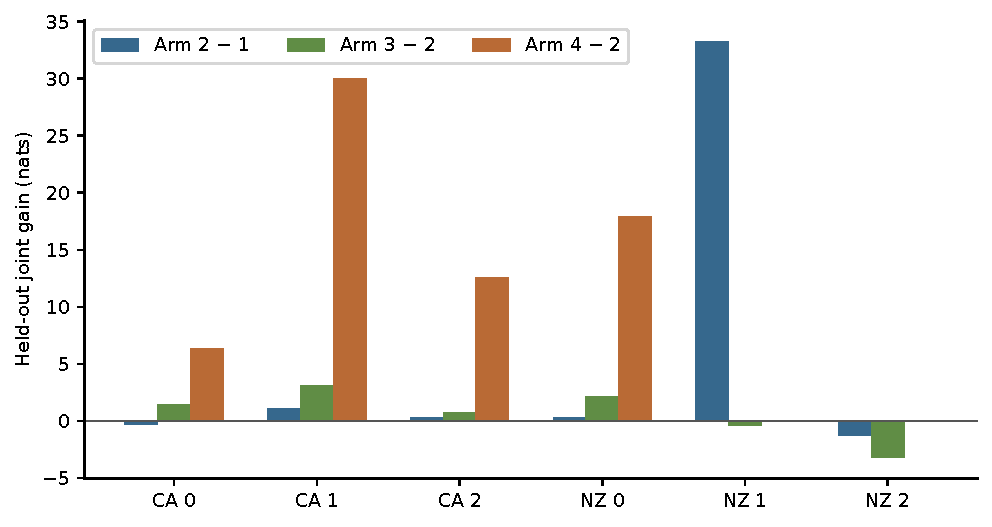
\includegraphics[width=\textwidth]{s03_completed_joint_contrasts.pdf}\caption{Saved held-out joint contrasts across all six folds. Each fold has its own refitted nuisance coefficients; these differences are not a causal mechanism decomposition. Saved custody checks and independent sampled raw validation passed.}\end{figure}
